
\begin{frame}[shrink]{Hoja de Ruta de Hoy}
  \vspace{4pt}
  \begin{center}
  \begin{tikzpicture}[
    node distance=0.25cm,
    roadstep/.style={rectangle, rounded corners=4pt, draw=arcaRed, fill=arcaRed!8,
                 minimum width=11.5cm, minimum height=0.55cm,
                 font=\footnotesize\bfseries\color{arcaDark}, align=left,
                 text width=10.5cm, inner sep=4pt},
    num/.style={circle, fill=arcaRed, text=white, font=\scriptsize\bfseries,
                minimum size=0.45cm, inner sep=0pt},
  ]
    \node[roadstep] (s0) {\hspace{0.7cm}Cierre clase 26: bajar dataset con \texttt{label-studio-sdk}};
    \node[roadstep, below=of s0] (s1) {\hspace{0.7cm}Estructura YOLO: carpetas + \texttt{data.yaml}};
    \node[roadstep, below=of s1] (s2) {\hspace{0.7cm}API de YOLO en profundidad (predict, track, export)};
    \node[roadstep, below=of s2] (s3) {\hspace{0.7cm}OCR formal: EasyOCR por dentro};
    \node[roadstep, below=of s3] (s4) {\hspace{0.7cm}Stack funcional + m\'etricas end-to-end};
    \node[roadstep, below=of s4] (s5) {\hspace{0.7cm}\textbf{Brain Tumor Detection:} m\'etricas medical-aware};
    \node[roadstep, below=of s5] (s6) {\hspace{0.7cm}\textbf{Package Segmentation:} API + m\'etricas de m\'ascara};

    \foreach \i in {0,...,6}{
      \node[num] at ([xshift=0.4cm]s\i.west) {\the\numexpr\i+1};
    }
  \end{tikzpicture}
  \end{center}
\end{frame}

% =============================================================================
%  BLOQUE 1: CIERRE CLASE 26 — LABEL STUDIO SDK
% =============================================================================
\sectionframe{Cierre Clase 26}{Bajar dataset de Label Studio con la librer\'ia oficial}

\begin{frame}[fragile,shrink]{C\'odigo: Bajar Dataset con SDK}
  \vspace{-4pt}
  \begin{pyblock}
!pip install -q label-studio-sdk

from label_studio_sdk import LabelStudio

# 1. Conectar (el SDK maneja el refresh token automaticamente)
ls = LabelStudio(
    base_url="https://label-studio-production-281f.up.railway.app",
    api_key=LS_TOKEN,
)

# 2. Listar proyectos
for p in ls.projects.list():
    print(f"  ID {p.id}: {p.title} ({p.task_number} tasks)")

# 3. Crear y descargar export en YOLO format
export = ls.projects.exports.create(
    project_id=1,
    export_type="YOLO",
)
ls.projects.exports.download(
    project_id=1, export_pk=export.id,
    save_path="dataset_ls.zip",
)
  \end{pyblock}
\end{frame}

% =============================================================================
%  BLOQUE 2: ESTRUCTURA YOLO
% =============================================================================
\sectionframe{Estructura YOLO}{C\'omo organizar el dataset y el \texttt{data.yaml}}

\begin{frame}[shrink]{La Anatom\'ia del Dataset}
  \vspace{4pt}
  \begin{center}
    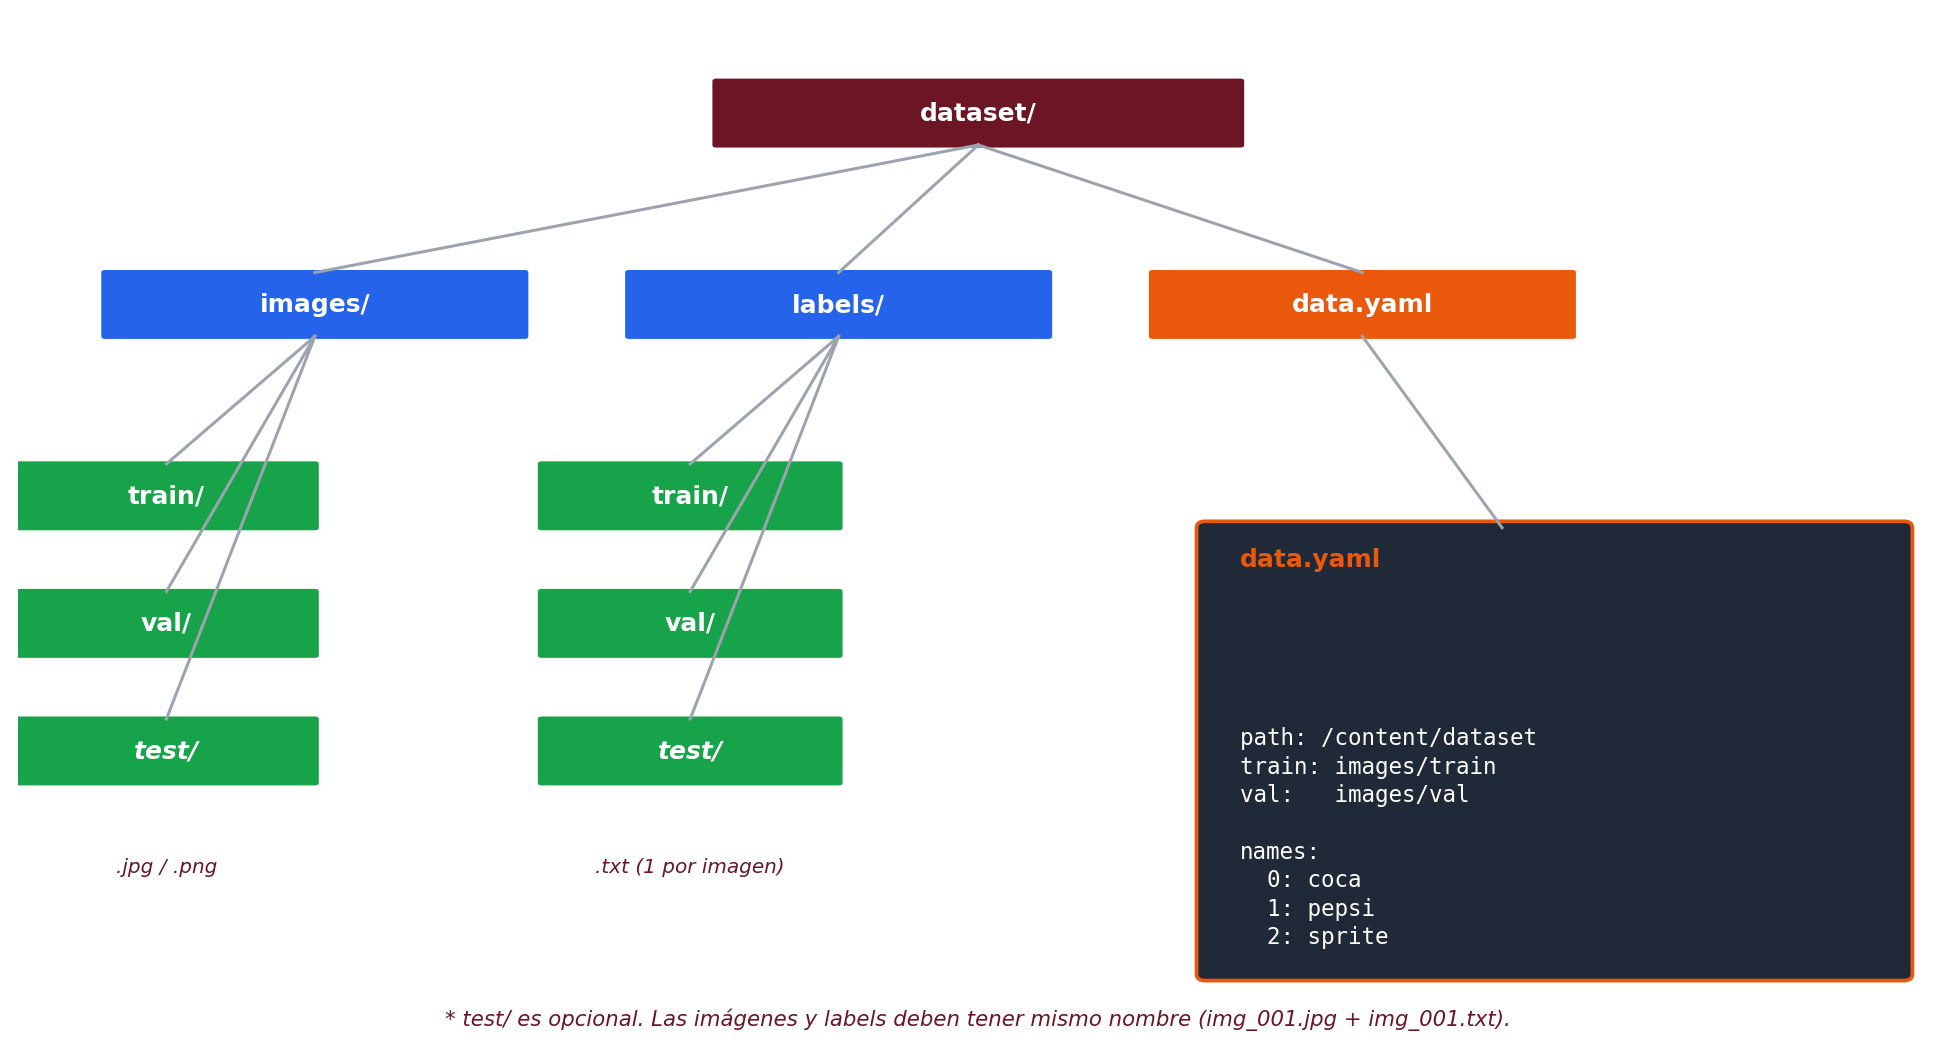
\includegraphics[width=0.92\textwidth]{fig_yolo_folder.png}
  \end{center}

  \vspace{4pt}
  {\scriptsize\color{textMuted}
    \faLightbulb\hspace{4pt} Ultralytics espera \emph{exactamente} este
    layout. Mismo nombre entre \texttt{images/} y \texttt{labels/}
    (\texttt{img\_001.jpg} $\leftrightarrow$ \texttt{img\_001.txt}).
    \texttt{test/} es opcional.}
\end{frame}

\begin{frame}[shrink]{El Archivo \texttt{data.yaml} Paso a Paso}
  \vspace{6pt}
  {\footnotesize
  \begin{tabular}{@{}p{2.5cm} p{9.5cm}@{}}
    \toprule
    \textbf{Campo} & \textbf{Qu\'e hace} \\
    \midrule
    \rowcolor{arcaGray}
    \texttt{path:}
    & Ruta absoluta a la carpeta ra\'iz del dataset. \\
    \texttt{train:}
    & Ruta a las im\'agenes de train, \emph{relativa a path}. Sin barra inicial. \\
    \rowcolor{arcaGray}
    \texttt{val:}
    & Igual pero para validaci\'on. \\
    \texttt{test:}
    & (opcional) Para evaluaci\'on final. \\
    \rowcolor{arcaGray}
    \texttt{names:}
    & Diccionario \texttt{\{class\_id: nombre\}}. Las claves son enteros 0..N. \\
    \texttt{nc:}
    & (legacy) N\'umero de clases. Ya no es necesario, se infiere de \texttt{names}. \\
    \bottomrule
  \end{tabular}
  }

  \vspace{10pt}
  \begin{tcolorbox}[colback=arcaRed!8, colframe=arcaRed, boxrule=0.5pt,
    arc=2pt, left=6pt, right=6pt, top=4pt, bottom=4pt]
    {\scriptsize\color{arcaDark}
    \faExclamationTriangle\hspace{4pt} Los \texttt{class\_id} en los archivos
    \texttt{.txt} deben coincidir EXACTAMENTE con los del \texttt{data.yaml}.
    Si \texttt{names: \{0: coca, 1: pepsi\}} pero el txt dice clase \texttt{2},
    el modelo nunca aprende.}
  \end{tcolorbox}
\end{frame}

\begin{frame}[fragile,shrink]{Formato de los \texttt{.txt}}
  \vspace{-4pt}
  \begin{pyblock}
# Cada imagen tiene un .txt asociado (mismo nombre):
#   images/train/img_001.jpg
#   labels/train/img_001.txt

# El .txt tiene UNA LINEA POR OBJETO:
# <class_id> <cx> <cy> <w> <h>
# todas las coordenadas normalizadas [0, 1]
# cx, cy = centro de la caja
# w, h   = ancho y alto

# Ejemplo (3 productos en una foto):
0 0.453 0.612 0.087 0.234     # class 0 (coca), centro (45.3%, 61.2%)
1 0.581 0.598 0.091 0.225     # class 1 (pepsi)
0 0.712 0.605 0.084 0.231     # otra coca
  \end{pyblock}

  \vspace{4pt}
  {\scriptsize\color{textMuted}
    \faLightbulb\hspace{4pt} Label Studio exporta justo as\'i.
    Si las cajas vienen en p\'ixeles absolutos, hay que normalizar
    dividiendo por (ancho, alto) de la imagen.}
\end{frame}

% =============================================================================
%  BLOQUE 3: API DE YOLO EN PROFUNDIDAD
% =============================================================================
\sectionframe{API de YOLO en Python}{predict, track, export — cada uno con su uso}

\begin{frame}[shrink]{Los 4 M\'etodos Principales de Ultralytics}
  \vspace{8pt}
  {\footnotesize
  \begin{tabular}{@{}p{2.5cm} p{4.5cm} p{5.5cm}@{}}
    \toprule
    \textbf{M\'etodo} & \textbf{Qu\'e hace} & \textbf{Cu\'ando usarlo} \\
    \midrule
    \rowcolor{arcaGray}
    \texttt{model.predict()}
    & Inferencia: detectar en imagen/video
    & Lo que usamos siempre, default \\
    \texttt{model.track()}
    & Predict + tracking de IDs entre frames
    & Conteo en video (no contar 2 veces el mismo objeto) \\
    \rowcolor{arcaGray}
    \texttt{model.train()}
    & Fine-tune con tu dataset
    & Una vez por proyecto \\
    \texttt{model.export()}
    & Convertir a ONNX, TFLite, CoreML, TensorRT
    & Para desplegar fuera de Python \\
    \bottomrule
  \end{tabular}
  }

  \vspace{12pt}
  \begin{tcolorbox}[colback=codeGreen!8, colframe=codeGreen, boxrule=0.5pt,
    arc=2pt, left=6pt, right=6pt, top=4pt, bottom=4pt]
    {\scriptsize\color{arcaDark}
    \faKey\hspace{4pt}\textbf{En esta clase:} usamos \texttt{predict()} para
    inferir, \texttt{train()} para fine-tune, y veremos \texttt{track()} en
    el caso de video.}
  \end{tcolorbox}
\end{frame}

\begin{frame}[fragile,shrink]{Predict con Todas Sus Opciones}
  \vspace{-4pt}
  \begin{pyblock}
results = model.predict(
    source="auto.jpg",        # imagen, video, URL, ndarray, lista
    conf=0.25,                # umbral confianza
    iou=0.7,                  # umbral NMS
    imgsz=640,                # resolucion
    classes=[0, 2],           # filtrar solo ciertas clases
    device="cuda",            # cpu / cuda / mps / 0,1,2 (multi-gpu)
    save=True,                # guarda imagen anotada
    save_txt=True,            # guarda labels en formato YOLO
    save_conf=True,           # incluye confianza en el txt
    save_crop=True,           # guarda cada deteccion como imagen separada
    project="runs", name="exp1",
    stream=False,             # True = generator (videos largos)
    verbose=False,
)
  \end{pyblock}

  \vspace{4pt}
  {\scriptsize\color{textMuted}
    \faLightbulb\hspace{4pt} \texttt{save\_crop=True} es \'util en pipeline OCR:
    YOLO ya te deja cada placa recortada en disco, lista para EasyOCR.}
\end{frame}

\begin{frame}[fragile,shrink]{Tracking para Video (Conteo Sin Duplicados)}
  \vspace{-4pt}
  \begin{pyblock}
# track() asocia un ID persistente a cada objeto entre frames.
# Sin track, "este carro" en el frame 1 y "este carro" en el frame 2
# serian 2 detecciones distintas → conteo inflado.

results = model.track(
    source="traffic.mp4",
    tracker="bytetrack.yaml",   # algoritmo (ByteTrack o BoT-SORT)
    persist=True,               # mantener IDs entre llamadas
    save=True,
)

# Cada deteccion ahora tiene id_int
for box in results[0].boxes:
    track_id = int(box.id[0]) if box.id is not None else None
    nombre = results[0].names[int(box.cls[0])]
    print(f"obj {track_id}: {nombre}")
  \end{pyblock}
\end{frame}

\begin{frame}[fragile,shrink]{Export: Sacar el Modelo de Python}
  \vspace{-4pt}
  \begin{pyblock}
# Una vez fine-tuneado, exportar para deploy donde no haya Python:
model.export(format="onnx")        # universal, runtime en C++/Java/JS
model.export(format="tflite")      # movil Android (lite)
model.export(format="coreml")      # iOS / Mac
model.export(format="engine")      # TensorRT (NVIDIA Jetson, max speed)

# Cada uno se carga distinto en su destino:
#   ONNX:    onnxruntime.InferenceSession("best.onnx")
#   TFLite:  tflite.Interpreter(model_path="best.tflite")
  \end{pyblock}

  \vspace{4pt}
  {\scriptsize\color{textMuted}
    \faLightbulb\hspace{4pt} Para producci\'on: \textbf{ONNX} es lo m\'as
    portable. Para edge real-time: \textbf{TensorRT} en una Jetson Nano da
    60+ FPS con yolo26n.}
\end{frame}

% =============================================================================
%  BLOQUE 4: OCR FORMAL
% =============================================================================
\sectionframe{OCR Formal}{Qu\'e es, c\'omo evolucion\'o, c\'omo funciona EasyOCR}

\begin{frame}[shrink]{?`Qu\'e Es OCR?}
  \vspace{6pt}
  {\footnotesize\color{arcaDark}\bfseries
    \textbf{Optical Character Recognition}: convertir im\'agenes de
    texto en cadenas de texto editables. Es la \emph{tarea de visi\'on}
    m\'as antigua con \'exito comercial.}

  \vspace{14pt}
  {\footnotesize
  \begin{itemize}\setlength{\itemsep}{6pt}
    \item[{\color{arcaRed}\scriptsize\faArrowRight}]
      \textbf{1950s:} primeros lectores de cheques bancarios (CMC-7,
      caracteres magn\'eticos).
    \item[{\color{arcaRed}\scriptsize\faArrowRight}]
      \textbf{1985--2005:} \textbf{Tesseract} (HP, luego Google):
      reglas + clasificador. A\'un se usa.
    \item[{\color{arcaRed}\scriptsize\faArrowRight}]
      \textbf{2015+:} OCR con deep learning (CRNN, attention).
    \item[{\color{arcaRed}\scriptsize\faArrowRight}]
      \textbf{2020:} \textbf{EasyOCR} (JaidedAI) y \textbf{PaddleOCR}
      (Baidu) democratizan deep OCR.
    \item[{\color{codeGreen}\scriptsize\faArrowRight}]
      \textbf{2023+:} OCR multimodal (GPT-4V, Claude Vision) lee texto
      \emph{en contexto}, pero son APIs pagas y m\'as lentas.
  \end{itemize}
  }
\end{frame}

\begin{frame}[shrink]{EasyOCR Por Dentro: 2 Modelos Encadenados}
  \vspace{4pt}
  \begin{center}
    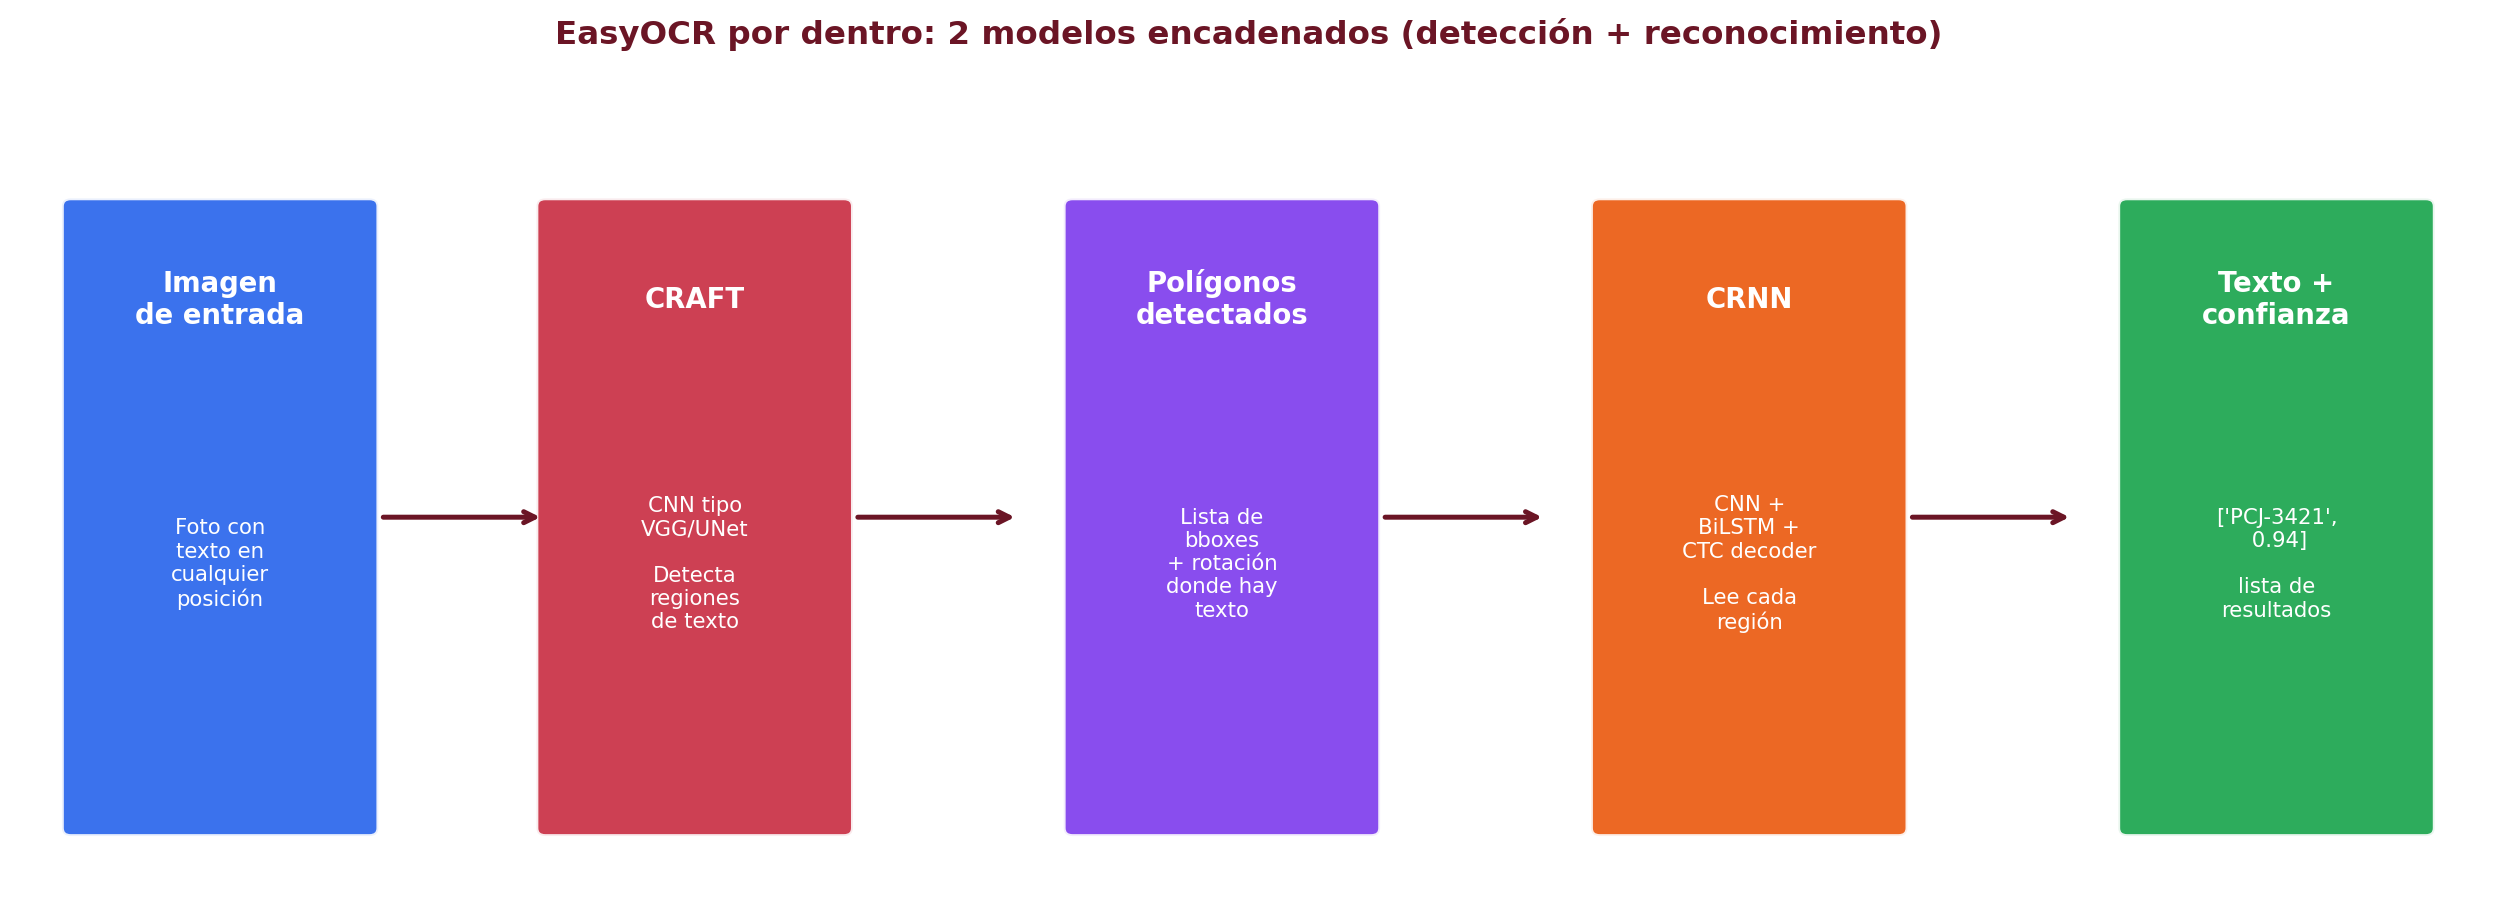
\includegraphics[width=0.95\textwidth]{fig_easyocr_pipeline.png}
  \end{center}

  \vspace{4pt}
  {\scriptsize\color{textMuted}
    \faLightbulb\hspace{4pt} \textbf{CRAFT} encuentra D\'ONDE est\'a el texto
    (regiones poligonales). \textbf{CRNN} lee QU\'E dice cada regi\'on.
    Cada uno es una red dedicada, entrenable por separado.}
\end{frame}

\begin{frame}[shrink]{Etapa 1: CRAFT --- Detecci\'on de Texto}
  \vspace{6pt}
  {\footnotesize\color{arcaDark}\bfseries
    \emph{Character Region Awareness for Text Detection}.
    Una CNN tipo VGG/UNet que predice 2 heatmaps por pixel:}

  \vspace{12pt}
  {\footnotesize
  \begin{itemize}\setlength{\itemsep}{6pt}
    \item[{\color{arcaRed}\scriptsize\faArrowRight}]
      \textbf{Region score} (cu\'al pixel es centro de un car\'acter)
    \item[{\color{arcaRed}\scriptsize\faArrowRight}]
      \textbf{Affinity score} (qu\'e tanto un pixel ``une'' caracteres
      adyacentes)
    \item[{\color{arcaRed}\scriptsize\faArrowRight}]
      Post-procesamiento: agrupar caracteres conectados $\to$ pol\'igonos
      alrededor del texto. Maneja texto inclinado, curvo, vertical.
    \item[{\color{codeGreen}\scriptsize\faArrowRight}]
      Output: lista de pol\'igonos donde hay texto.
  \end{itemize}
  }

  \vspace{8pt}
  {\scriptsize\color{textMuted}
    \faLightbulb\hspace{4pt} Esta etapa la pueden saltar si ya recortaron la
    regi\'on (ej. YOLO les dio el bbox de la placa). EasyOCR re-detecta
    igual, es r\'apido en crops chicos.}
\end{frame}

\begin{frame}[shrink]{Etapa 2: CRNN --- Reconocimiento de Caracteres}
  \vspace{6pt}
  {\footnotesize\color{arcaDark}\bfseries
    \emph{Convolutional Recurrent Neural Network}. Para cada regi\'on
    detectada, lee la secuencia de caracteres:}

  \vspace{12pt}
  {\footnotesize
  \begin{enumerate}\setlength{\itemsep}{6pt}
    \item[{\color{arcaRed}\bfseries 1.}]
      \textbf{CNN}: extrae features visuales de la regi\'on de texto
      (como cualquier CNN).
    \item[{\color{arcaRed}\bfseries 2.}]
      \textbf{BiLSTM}: trata los features como una \emph{secuencia
      temporal} (lectura de izquierda a derecha) y modela
      dependencias entre caracteres.
    \item[{\color{arcaRed}\bfseries 3.}]
      \textbf{CTC decoder}: alinea los outputs del LSTM con los
      caracteres reales \emph{sin importar el largo}. La parte que
      permite ``placa de 6 letras'' o ``placa de 8 letras'' con la
      misma red.
    \item[{\color{codeGreen}\bfseries 4.}]
      Output: cadena de texto + confianza.
  \end{enumerate}
  }
\end{frame}

\begin{frame}[fragile,shrink]{API de EasyOCR --- Todos los Par\'ametros}
  \vspace{-4pt}
  \begin{pyblock}
import easyocr

# 1. Crear reader (descarga modelos la 1ra vez)
reader = easyocr.Reader(
    ['en', 'es'],            # idiomas (multi-idioma OK)
    gpu=True,                # acelera 5-10x
    detect_network="craft",  # detector (craft o dbnet18)
    recog_network="standard",# reconocedor (standard, latin_g2, ...)
    model_storage_directory="/tmp/easyocr",
)

# 2. Leer texto
result = reader.readtext(
    crop,
    detail=1,           # 1=bbox+texto+conf, 0=solo texto
    paragraph=False,    # True agrupa parrafos
    allowlist="0123456789ABCDEFGHIJKLMNOPQRSTUVWXYZ-",
    min_size=10,        # ignora textos < N pixeles
    low_text=0.4,       # umbral region score
    link_threshold=0.4, # umbral affinity score
    decoder="greedy",   # greedy, beamsearch, wordbeamsearch
    beamWidth=5,        # ancho del beam si decoder=beamsearch
)
  \end{pyblock}
\end{frame}

\begin{frame}[shrink]{Cu\'ando EasyOCR vs Alternativas}
  \vspace{8pt}
  {\footnotesize
  \begin{tabular}{@{}p{2.8cm} p{4.2cm} p{5.0cm}@{}}
    \toprule
    \textbf{Herramienta} & \textbf{Fuerza} & \textbf{Cu\'ando usarla} \\
    \midrule
    \rowcolor{arcaGray}
    \textbf{EasyOCR}
    & Balance precision/velocidad, 80+ idiomas
    & \textbf{Default razonable} para casi todo \\
    Tesseract
    & R\'apido en CPU, maduro (1985+)
    & Docs escaneados con texto limpio \\
    \rowcolor{arcaGray}
    PaddleOCR
    & 3-5$\times$ m\'as r\'apido, m\'as preciso en chino
    & Producci\'on a escala \\
    TrOCR (Microsoft)
    & Transformer, mejor en manuscrito
    & Documentos escritos a mano \\
    \rowcolor{arcaGray}
    GPT-4V / Claude Vision
    & Lee texto + entiende contexto
    & Documentos complejos, formularios \\
    Cloud OCR (AWS Textract, Google Vision)
    & API gestionada, soporte enterprise
    & Cuando no quieres mantener modelos \\
    \bottomrule
  \end{tabular}
  }
\end{frame}

% =============================================================================
%  BLOQUE 5: STACK + METRICAS
% =============================================================================
\sectionframe{Stack Funcional}{Pipeline LPR end-to-end + m\'etricas}

\begin{frame}[shrink]{Stack del LPR (Lectura de Placas)}
  \vspace{4pt}
  \begin{center}
    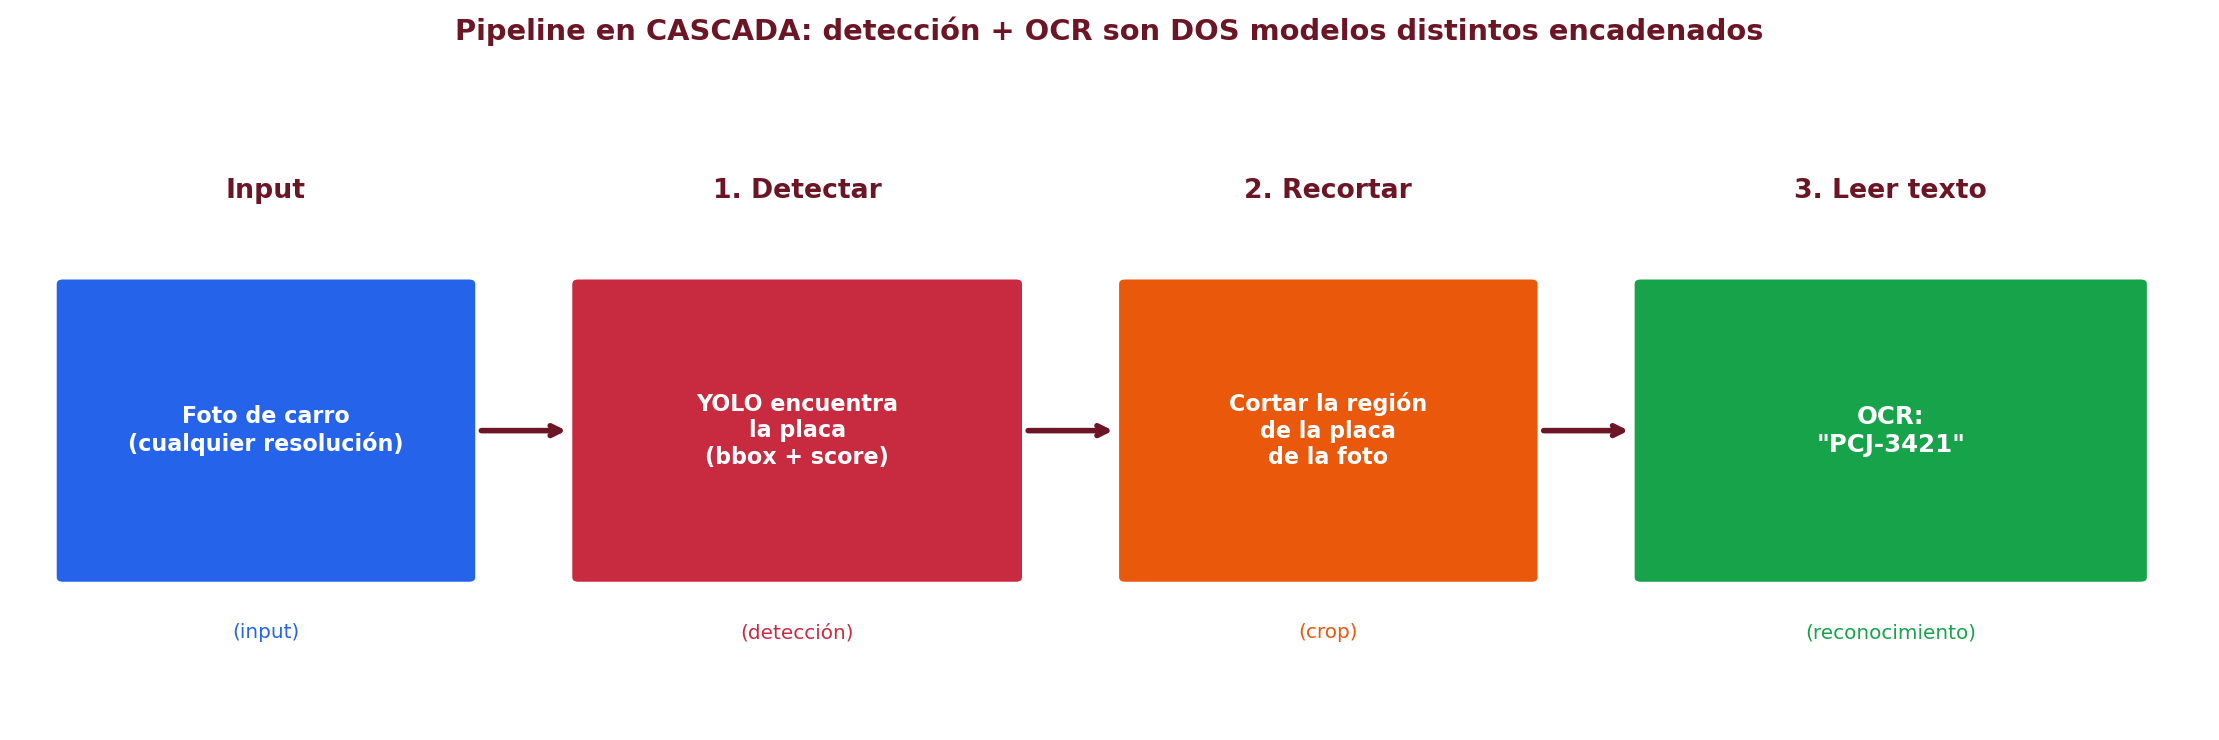
\includegraphics[width=0.95\textwidth]{fig_ocr_cascade_diagram.png}
  \end{center}

  \vspace{4pt}
  {\scriptsize\color{textMuted}
    \faLightbulb\hspace{4pt} Es la composici\'on de \textbf{2 modelos}:
    YOLO fine-tuneado encuentra la placa, EasyOCR lee el texto.
    Cada uno tiene su tarea y se eval\'ua independiente.}
\end{frame}

\begin{frame}[shrink]{M\'etricas End-to-End}
  \vspace{8pt}
  {\footnotesize
  \begin{tabular}{@{}p{3.0cm} p{4.0cm} p{5.0cm}@{}}
    \toprule
    \textbf{Etapa} & \textbf{M\'etrica} & \textbf{Objetivo} \\
    \midrule
    \rowcolor{arcaGray}
    Detecci\'on (YOLO)
    & mAP@0.5
    & $\geq$ 0.85 \\
    Detecci\'on (YOLO)
    & Precision / Recall
    & Ambos $\geq$ 0.85 \\
    \rowcolor{arcaGray}
    Reconocimiento (OCR)
    & \textbf{CER} (Character Error Rate)
    & $\leq$ 0.05 (errores por car\'acter) \\
    Reconocimiento (OCR)
    & \textbf{Accuracy exacto}
    & $\geq$ 0.90 (placas le\'idas perfectas) \\
    \rowcolor{arcaGray}
    Pipeline completo
    & Latencia
    & $<$ 500 ms por imagen \\
    Pipeline completo
    & End-to-end accuracy
    & $\geq$ 0.80 \\
    \bottomrule
  \end{tabular}
  }

  \vspace{10pt}
  \begin{tcolorbox}[colback=arcaGray, colframe=arcaRed, boxrule=0.5pt,
    arc=2pt, left=6pt, right=6pt, top=4pt, bottom=4pt]
    {\scriptsize\color{arcaDark}
    \faKey\hspace{4pt} \textbf{CER} = caracteres mal le\'idos $/$ caracteres
    totales. Es la m\'etrica est\'andar de OCR. Ej: ``PCJ-3421'' vs
    ``PCJ-3471'' $\to$ 1 error de 8 $\to$ CER = 0.125.}
  \end{tcolorbox}
\end{frame}

% =============================================================================
%  BLOQUE 6: BRAIN TUMOR — DETECCION CON METRICAS MEDICAL-AWARE
% =============================================================================
\sectionframe{Brain Tumor Detection}{Detecci\'on en MRI + por qu\'e la m\'etrica depende del dominio}

\begin{frame}[shrink]{El Contexto: Detecci\'on Asistida en MRI}
  \vspace{6pt}
  {\footnotesize\color{arcaDark}\bfseries
    Una cl\'inica tiene cientos de res\'oncias magn\'eticas (MRI) cerebrales
    pendientes de revisi\'on. Buscan un modelo que pre-filtre las
    im\'agenes sospechosas de tumor para que el radi\'ologo solo dedique
    tiempo a las que tienen probabilidad alta.}

  \vspace{12pt}
  {\footnotesize
  \begin{itemize}\setlength{\itemsep}{5pt}
    \item[{\color{arcaRed}\scriptsize\faArrowRight}]
      Misma t\'ecnica que placas: detection con bbox. Pero las
      \emph{prioridades} de negocio cambian.
    \item[{\color{arcaRed}\scriptsize\faArrowRight}]
      Dataset: \texttt{brain-tumor} de Ultralytics. 893 train + 223
      val. 2 clases: \texttt{negative} (no tumor) y \texttt{positive}
      (tumor).
    \item[{\color{codeGreen}\scriptsize\faArrowRight}]
      Lo subimos a Label Studio con 80\% pre-etiquetado (ground truth
      real) y 20\% vac\'io para que el equipo lo termine.
  \end{itemize}
  }
\end{frame}

\begin{frame}[shrink]{Placas vs Brain Tumor: la M\'etrica Cambia}
  \vspace{10pt}
  {\footnotesize
  \begin{tabular}{@{}p{4.0cm} p{4.0cm} p{4.0cm}@{}}
    \toprule
    & \textbf{Placas (LPR)} & \textbf{Brain Tumor} \\
    \midrule
    \rowcolor{arcaGray}
    M\'etrica que importa
    & \textbf{Precision}
    & \textbf{Recall (Sensitivity)} \\
    ?`Qu\'e duele m\'as?
    & Leer una placa que no existe
    & \textbf{Perder un tumor real} \\
    \rowcolor{arcaGray}
    Dominio del etiquetador
    & Cualquier persona
    & \textbf{Radi\'ologo} \\
    Costo de etiquetar
    & $\sim$10 segundos
    & \textbf{Minutos por imagen} \\
    \rowcolor{arcaGray}
    \texttt{conf} \'optimo
    & Alto ($\sim$0.5)
    & \textbf{Bajo ($\sim$0.15)} \\
    \bottomrule
  \end{tabular}
  }

  \vspace{14pt}
  \begin{tcolorbox}[colback=arcaRed!8, colframe=arcaRed, boxrule=0.5pt,
    arc=2pt, left=6pt, right=6pt, top=4pt, bottom=4pt]
    {\scriptsize\color{arcaDark}
    \faKey\hspace{4pt}\textbf{Regla:} la m\'etrica no la elige el modelo,
    la elige \emph{el costo} de un falso positivo vs un falso negativo
    en tu dominio. Decide primero, optimiza despu\'es.}
  \end{tcolorbox}
\end{frame}

\begin{frame}[shrink]{Flujo del Etiquetado}
  \vspace{6pt}
  {\footnotesize\color{arcaDark}\bfseries
    El proyecto \texttt{Clase 27 - Brain Tumor Detection} en Label
    Studio tiene 893 tareas:}

  \vspace{10pt}
  {\footnotesize
  \begin{enumerate}\setlength{\itemsep}{5pt}
    \item \textbf{$\sim$715 ya etiquetadas} con la ground truth del
      dataset original (vienen como \emph{annotations}, no predictions,
      as\'i s\'i exportan a YOLO).
    \item \textbf{$\sim$180 sin etiquetar} para que cada equipo las complete.
      Instrucciones visibles en la UI del proyecto:
      \begin{itemize}\setlength{\itemsep}{2pt}
        \item Si se observa una regi\'on sospechosa: dibujar
          rect\'angulo con clase \texttt{positive}.
        \item Si la imagen se considera sin tumor: enviar (Submit) sin
          rect\'angulos.
      \end{itemize}
    \item Descargan el dataset completo con \texttt{label-studio-sdk}
      (mismo c\'odigo que usaron para placas).
    \item Entrenan \texttt{yolo26n.pt} con el conjunto resultante.
  \end{enumerate}
  }

  \vspace{6pt}
  \begin{tcolorbox}[colback=codeGreen!8, colframe=codeGreen, boxrule=0.5pt,
    arc=2pt, left=6pt, right=6pt, top=4pt, bottom=4pt]
    {\scriptsize\color{arcaDark}
    \faLightbulb\hspace{4pt}\textbf{Nota pedag\'ogica:} ning\'un
    estudiante es radi\'ologo, as\'i que las 180 nuevas bboxes ser\'an
    ruidosas. Esa es la lecci\'on principal: \emph{la calidad del
    etiquetador define el techo de tu modelo}. Compararemos m\'etricas
    antes y despu\'es de a\~nadir las nuevas anotaciones.}
  \end{tcolorbox}
\end{frame}

\begin{frame}[shrink]{M\'etricas en Detalle: Precision vs Recall}
  \vspace{6pt}
  {\footnotesize\color{arcaDark}\bfseries
    Cuando entrenan, YOLO reporta:}

  \vspace{10pt}
  {\footnotesize
  \begin{tabular}{@{}p{3.2cm} p{8.5cm}@{}}
    \toprule
    \textbf{M\'etrica} & \textbf{Qu\'e mide / cu\'ando importa} \\
    \midrule
    \rowcolor{arcaGray}
    \textbf{Precision}
    & TP / (TP + FP). De lo que llam\'e tumor, ?`qu\'e \% lo era?
      $\to$ pocas falsas alarmas. \\
    \textbf{Recall (Sensitivity)}
    & TP / (TP + FN). De los tumores reales, ?`qu\'e \% detect\'e?
      $\to$ no perderse casos. \\
    \rowcolor{arcaGray}
    \textbf{F1}
    & Media arm\'onica P y R. \'Util cuando ambos pesan parecido. \\
    \textbf{mAP@0.5}
    & Average Precision usando IoU $\geq$ 0.5. La m\'etrica de cabecera
      en detection. \\
    \rowcolor{arcaGray}
    \textbf{Confusion matrix}
    & C\'omo se confunde el modelo entre clases. En tumor: ver
      cu\'ando llama \texttt{negative} a un \texttt{positive}. \\
    \bottomrule
  \end{tabular}
  }

  \vspace{8pt}
  {\scriptsize\color{textMuted}
    \faLightbulb\hspace{4pt} Para subir recall en \texttt{predict()}:
    bajar \texttt{conf} (0.5 $\to$ 0.15). El modelo detecta m\'as, con
    m\'as ruido, pero pierde menos. El radi\'ologo descarta lo extra.}
\end{frame}

% =============================================================================
%  BLOQUE 7: SEGMENTACION
% =============================================================================
\sectionframe{Segmentaci\'on}{Cuando los bboxes no alcanzan}

\begin{frame}[shrink]{?`Por Qu\'e Necesitamos Segmentaci\'on?}
  \vspace{4pt}
  \begin{center}
    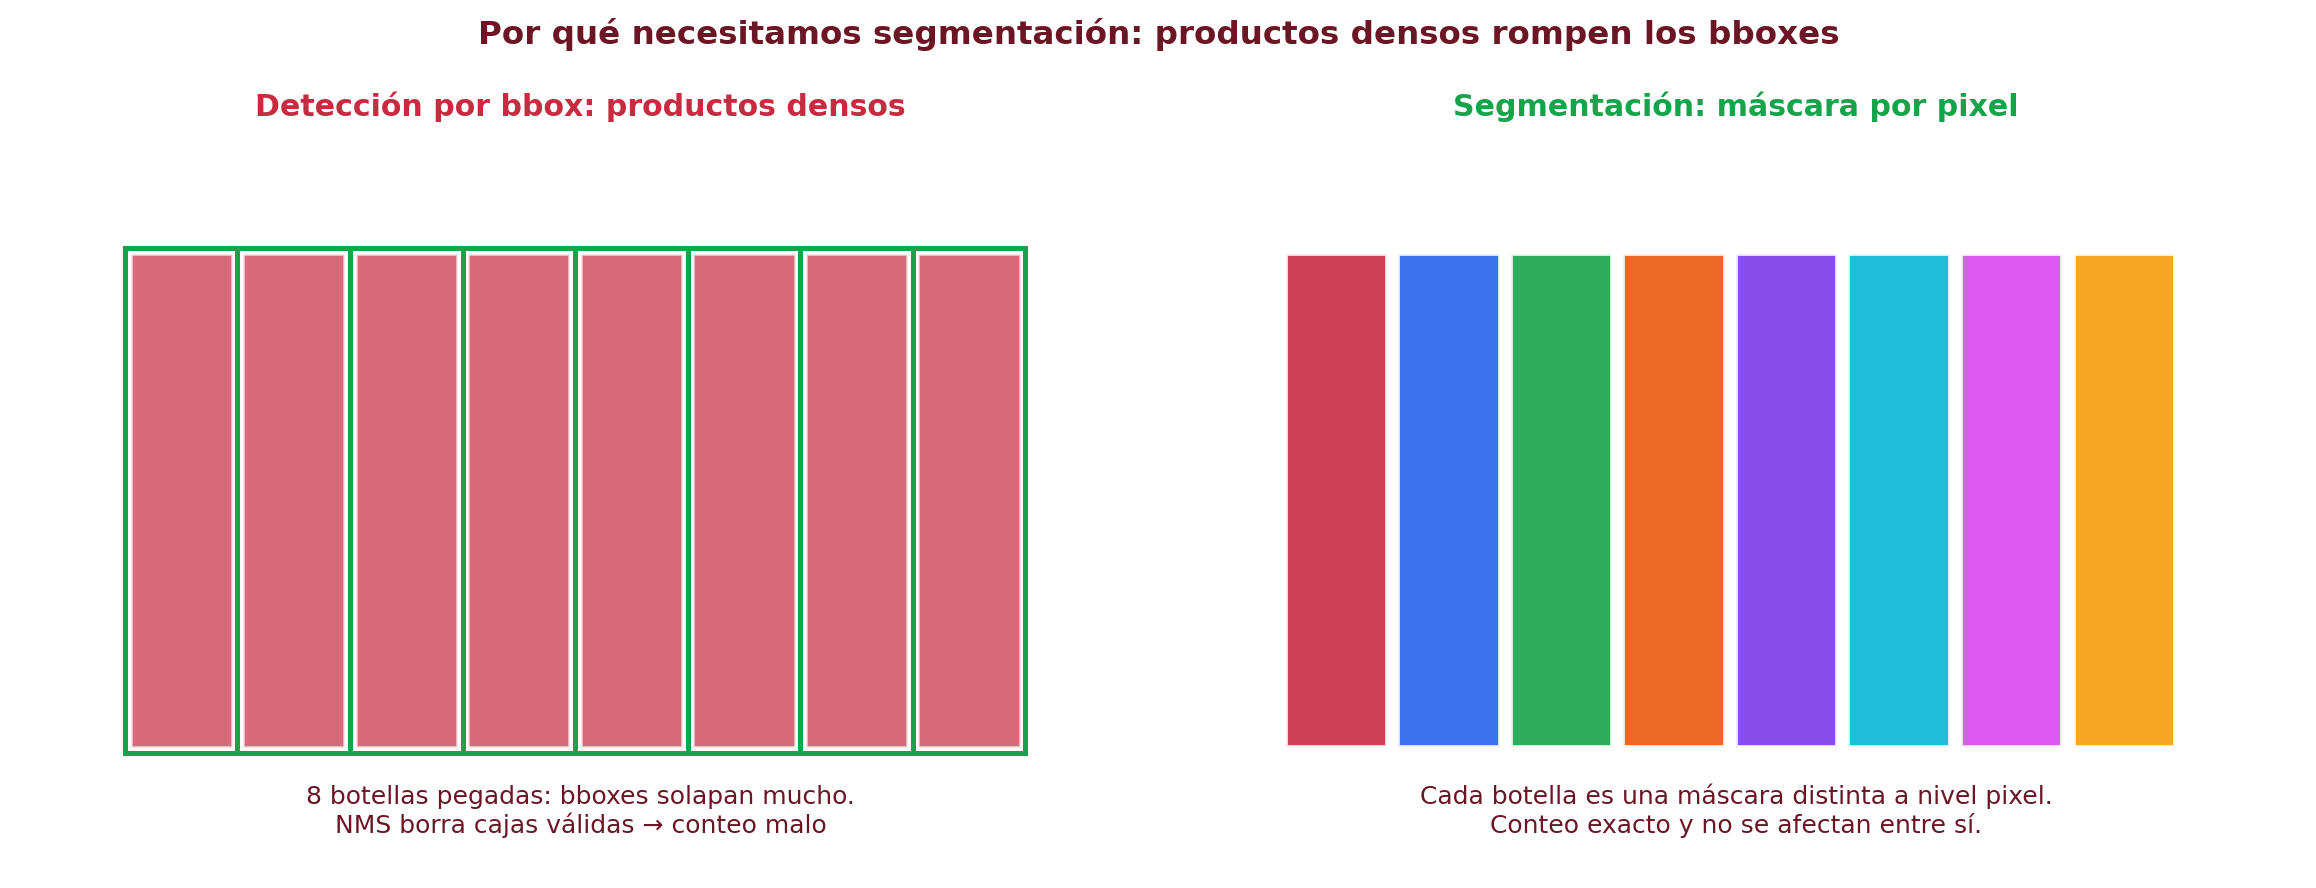
\includegraphics[width=0.95\textwidth]{fig_seg_motivacion.png}
  \end{center}

  \vspace{4pt}
  {\scriptsize\color{textMuted}
    \faLightbulb\hspace{4pt} En productos pegados, las bboxes solapan
    much\'isimo. NMS borra cajas v\'alidas. Con segmentaci\'on cada producto
    tiene su \emph{m\'ascara} a nivel pixel y no se confunden entre s\'i.}
\end{frame}

\begin{frame}[shrink]{Dos Tipos de Segmentaci\'on}
  \vspace{4pt}
  \begin{center}
    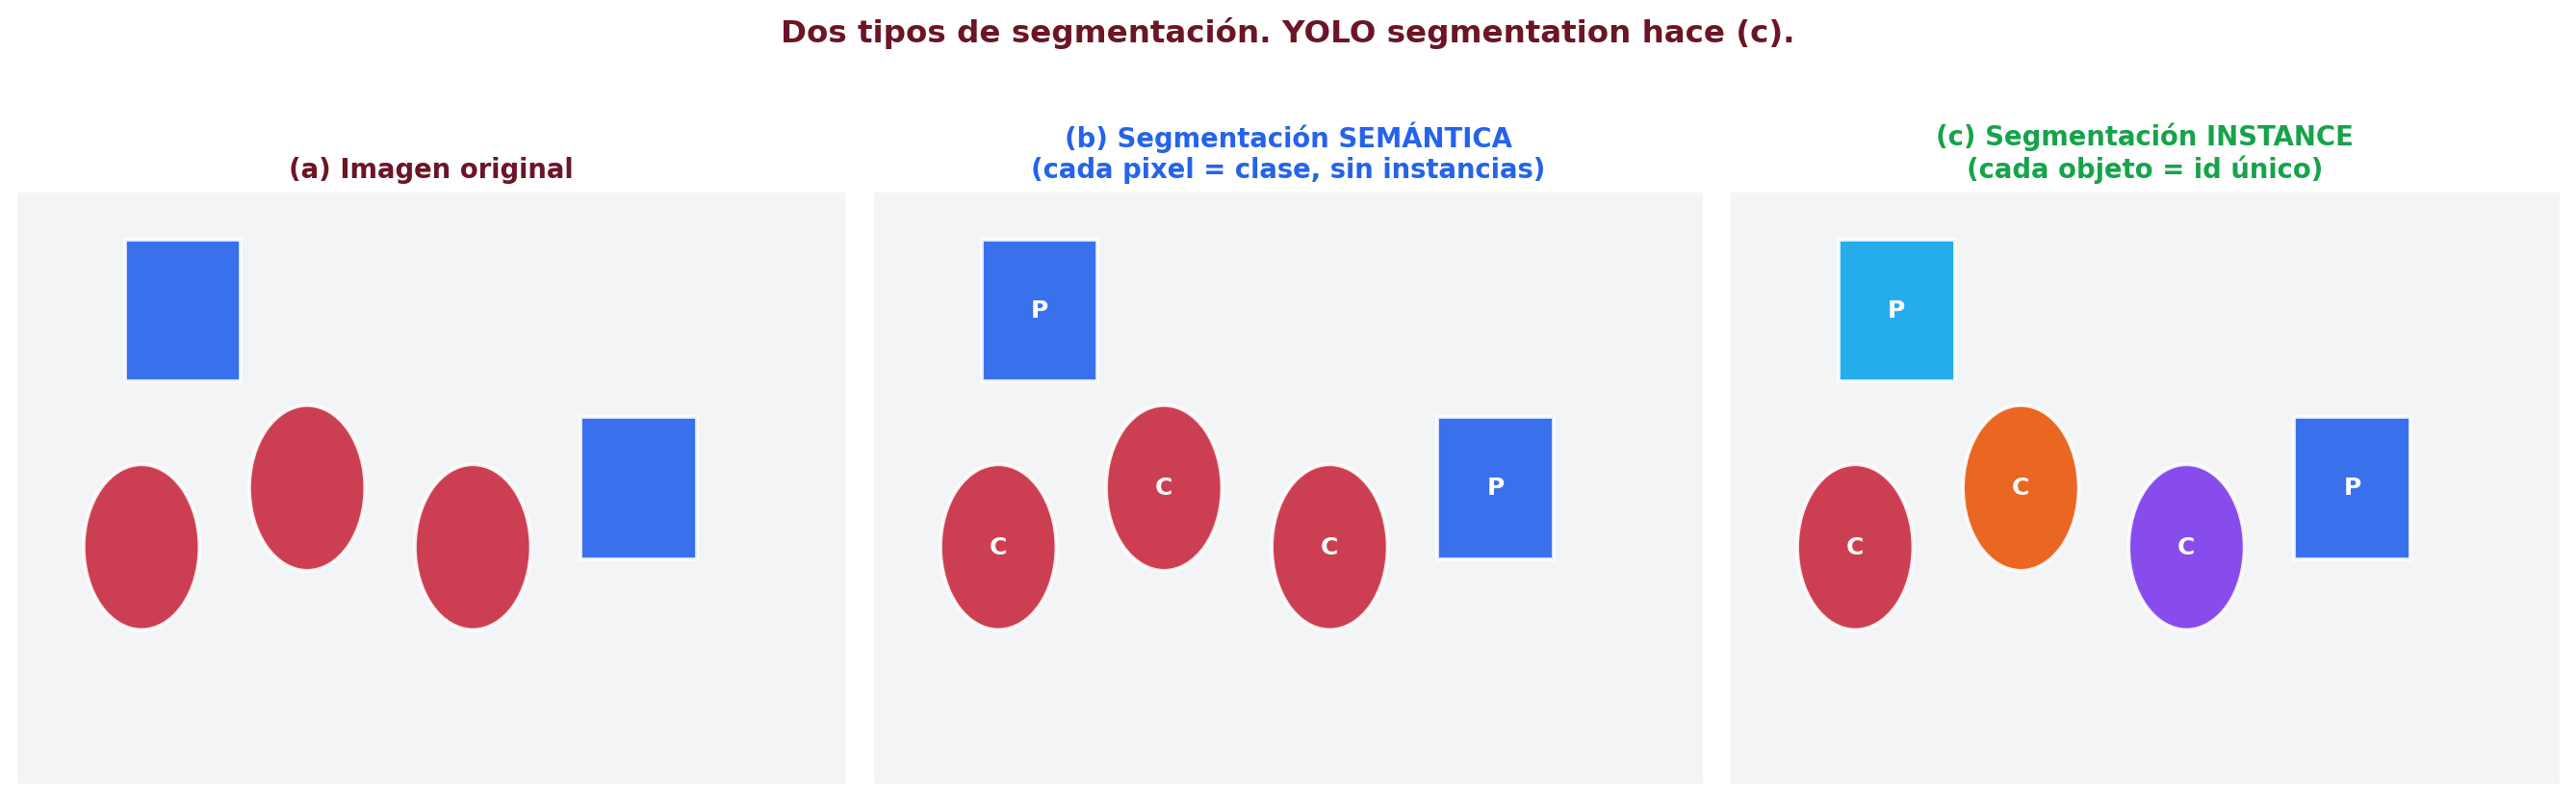
\includegraphics[width=0.97\textwidth]{fig_seg_types.png}
  \end{center}

  \vspace{4pt}
  {\footnotesize
  \begin{itemize}\setlength{\itemsep}{2pt}
    \item[{\color{arcaRed}\scriptsize\faArrowRight}]
      \textbf{Semantic:} cada pixel = una clase. Pero no distingue
      ``primera Coca'' de ``segunda Coca'' --- todas en rojo.
    \item[{\color{arcaRed}\scriptsize\faArrowRight}]
      \textbf{Instance:} cada pixel = clase \emph{m\'as} un ID \'unico.
      \textbf{Permite contar.}
    \item[{\color{codeGreen}\scriptsize\faArrowRight}]
      YOLO segmentation hace \textbf{instance segmentation}.
  \end{itemize}
  }
\end{frame}

\begin{frame}[fragile,shrink]{API de YOLO Segmentation}
  \vspace{-4pt}
  \begin{pyblock}
from ultralytics import YOLO

# Mismo patron, distinto modelo (sufijo -seg)
model = YOLO("yolo26n-seg.pt")     # n/s/m/l/x tambien existen

# Misma API que detection
results = model("cooler.jpg", conf=0.5)
res = results[0]

# AHORA hay 2 cosas:
boxes = res.boxes              # las cajas (como detection)
masks = res.masks              # NUEVO: mascaras por objeto

# Cada mascara es un tensor con la silueta del objeto
print(f"Detecciones: {len(boxes)}")
print(f"Mascaras shape: {masks.data.shape}")  # (N, H, W) — N mascaras binarias

# Visualizar como antes
res.plot()                     # dibuja bbox + mascara coloreada
  \end{pyblock}
\end{frame}

\begin{frame}[fragile]{Acceder a Cada M\'ascara}
  \vspace{-4pt}
  \begin{pyblock}
# Mascara = array binario del tamano de la imagen.
res = model("cooler.jpg")[0]

for i, mask in enumerate(res.masks.data):
    # mask: tensor (H, W) binario (0 o 1)
    area = mask.sum().item()
    clase = res.names[int(res.boxes.cls[i])]
    print(f"Obj {i}: {clase}, area = {area} px")

# Tambien como poligono (contorno):
for poly in res.masks.xy:
    print(f"Poligono con {len(poly)} puntos")
  \end{pyblock}
\end{frame}

\begin{frame}[shrink]{M\'etricas de Segmentaci\'on}
  \vspace{8pt}
  {\footnotesize
  \begin{tabular}{@{}p{3.0cm} p{4.5cm} p{4.7cm}@{}}
    \toprule
    \textbf{M\'etrica} & \textbf{Qu\'e mide} & \textbf{Cu\'ando importa} \\
    \midrule
    \rowcolor{arcaGray}
    \textbf{Mask IoU}
    & Intersecci\'on / uni\'on de \emph{pixeles} (no de cajas)
    & La m\'etrica base de segmentaci\'on \\
    \textbf{mAP-Mask@0.5}
    & Average Precision usando mask IoU $\geq$ 0.5
    & \textbf{La reina} en seg, an\'aloga a mAP-Box \\
    \rowcolor{arcaGray}
    \textbf{Dice / F1}
    & 2 $\cdot$ |A $\cap$ B| / (|A| + |B|)
    & Datasets m\'edicos, m\'as sensible que IoU \\
    \textbf{mIoU}
    & IoU promedio por clase
    & Semantic segmentation \\
    \rowcolor{arcaGray}
    \textbf{Pixel accuracy}
    & \% pixeles correctamente clasificados
    & Reporte simple, m\'as enga\~noso \\
    \bottomrule
  \end{tabular}
  }

  \vspace{8pt}
  {\scriptsize\color{textMuted}
    \faLightbulb\hspace{4pt} Ultralytics reporta \texttt{mAP@0.5-Mask}
    autom\'aticamente cuando entrenas con \texttt{*-seg.pt}.}
\end{frame}

\begin{frame}[shrink]{Mask IoU Visualmente}
  \vspace{4pt}
  \begin{center}
    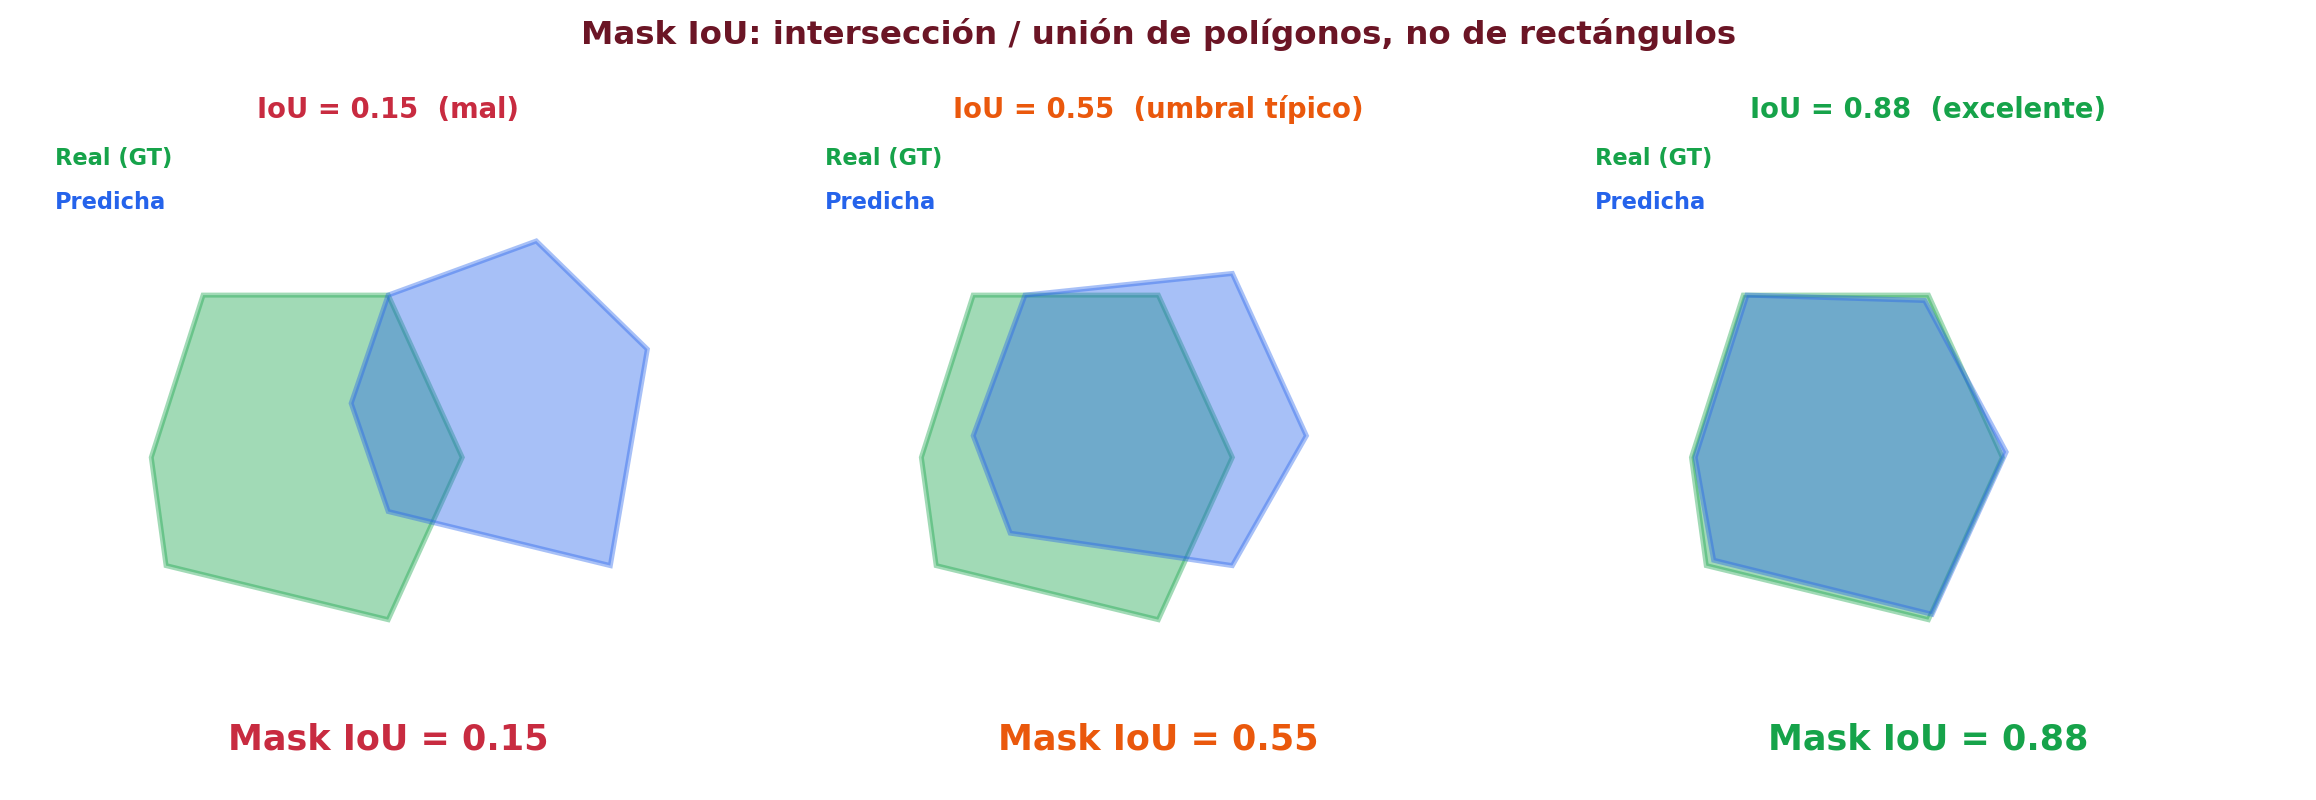
\includegraphics[width=0.95\textwidth]{fig_mask_iou.png}
  \end{center}

  \vspace{4pt}
  {\scriptsize\color{textMuted}
    \faLightbulb\hspace{4pt} Comparado con Box IoU (rectangulos), Mask
    IoU usa la silueta real $\to$ m\'etrica m\'as estricta y m\'as
    informativa cuando el objeto no es rectangular.}
\end{frame}

\begin{frame}[shrink]{Trade-offs Segmentaci\'on vs Detecci\'on}
  \vspace{8pt}
  {\footnotesize
  \begin{tabular}{@{}p{3.5cm} p{4.0cm} p{4.5cm}@{}}
    \toprule
    & \textbf{Detection (bbox)} & \textbf{Segmentation (mask)} \\
    \midrule
    \rowcolor{arcaGray}
    Etiquetado
    & R\'apido (4 clicks)
    & 5--10$\times$ m\'as lento (pol\'igono punto a punto) \\
    Tama\~no de modelo
    & yolo26n: 6 MB
    & yolo26n-seg: 7 MB \\
    \rowcolor{arcaGray}
    Velocidad inferencia
    & R\'apido
    & 10--20\% m\'as lento \\
    Precisi\'on en densidad
    & Cae con solape
    & \textbf{Mantiene precisi\'on} \\
    \rowcolor{arcaGray}
    Tipo de output
    & Rect\'angulo
    & Pol\'igono / m\'ascara \\
    \bottomrule
  \end{tabular}
  }

  \vspace{10pt}
  \begin{tcolorbox}[colback=codeGreen!8, colframe=codeGreen, boxrule=0.5pt,
    arc=2pt, left=6pt, right=6pt, top=4pt, bottom=4pt]
    {\scriptsize\color{arcaDark}
    \faKey\hspace{4pt}\textbf{Regla pr\'actica:} si los objetos no se solapan
    fuerte, usar detection (m\'as r\'apido de etiquetar y entrenar). Si se
    solapan mucho o necesitas \'area exacta, usar segmentation.}
  \end{tcolorbox}
\end{frame}

% ---------- Bloque 7: Package Segmentation ----------
\begin{frame}[shrink]{Problema: Conteo de Cajas en Pallets}
  \vspace{6pt}
  {\footnotesize\color{arcaDark}\bfseries
    Una bodega de distribuci\'on recibe pallets con cajas mezcladas.
    Quieren un sistema que \emph{cuente autom\'aticamente} las cajas
    para reconciliar inventario al recibir.}

  \vspace{12pt}
  {\footnotesize\color{arcaDark}\bfseries Por qu\'e segmentaci\'on y no detection:}

  \vspace{8pt}
  {\footnotesize
  \begin{itemize}\setlength{\itemsep}{5pt}
    \item[{\color{arcaRed}\scriptsize\faArrowRight}]
      Cajas \textbf{pegadas y apiladas} $\to$ bboxes solapan masivamente,
      NMS borra cajas v\'alidas.
    \item[{\color{arcaRed}\scriptsize\faArrowRight}]
      Necesitan medir \textbf{\'area} (caja grande vs chica) para
      inferir tama\~no/peso.
    \item[{\color{arcaRed}\scriptsize\faArrowRight}]
      Las cajas no son rectangulares en la imagen (perspectiva,
      rotaci\'on) $\to$ bbox malgasta \'area.
  \end{itemize}
  }
\end{frame}

\begin{frame}[shrink]{Dataset: Por Qu\'e No Usamos Label Studio Aqu\'i}
  \vspace{8pt}
  {\footnotesize\color{arcaDark}\bfseries
    \texttt{package-seg} de Ultralytics: 2197 im\'agenes, 1 clase
    (\texttt{package}). Auto-bajada con \texttt{data="package-seg.yaml"}.}

  \vspace{12pt}
  {\footnotesize
  \begin{itemize}\setlength{\itemsep}{6pt}
    \item[{\color{arcaRed}\scriptsize\faArrowRight}]
      Etiquetar 2200 pol\'igonos en LS: $\sim$5 min por imagen
      $\to$ \textbf{180 horas $=$ 4.5 semanas full-time} para una persona.
    \item[{\color{arcaRed}\scriptsize\faArrowRight}]
      Cuando existe un benchmark p\'ublico cercano a tu problema,
      \textbf{no etiquetes desde cero}. Empieza con el benchmark,
      mide, decide si necesitas tus propios datos.
    \item[{\color{codeGreen}\scriptsize\faArrowRight}]
      Lecci\'on opuesta al brain tumor: ah\'i ten\'iamos un dataset
      manejable y vali\'o la pena etiquetar; aqu\'i no.
  \end{itemize}
  }
\end{frame}

\begin{frame}[fragile,shrink]{Entrenar Package-Seg}
  \vspace{-4pt}
  \begin{pyblock}
from ultralytics import YOLO

# Mismo patron que detection, distinto modelo (-seg)
model = YOLO("yolo26n-seg.pt")

# Ultralytics resuelve el path solo, baja el dataset si falta
results = model.train(
    data="package-seg.yaml",   # ¡no es un path, es el nombre del YAML oficial!
    epochs=10,
    imgsz=640,
    batch=8,
    device="cuda",
)

# Validar
m = model.val(data="package-seg.yaml")
print(f"BBox mAP@0.5  = {m.box.map50:.3f}")
print(f"Mask mAP@0.5  = {m.seg.map50:.3f}")   # NUEVO: m\'etrica de mascara
  \end{pyblock}

  \vspace{4pt}
  {\scriptsize\color{textMuted}
    \faLightbulb\hspace{4pt} Ultralytics tiene varios YAMLs oficiales
    (\texttt{coco8}, \texttt{brain-tumor}, \texttt{package-seg}\ldots).
    Pasar el nombre dispara la descarga autom\'atica.}
\end{frame}
\sectionframe{Cierre}{Lo que aprendimos hoy y qu\'e viene}

\begin{frame}[shrink]{Resumen}
  \vspace{6pt}
  \begin{columns}[T]
    \begin{column}{0.48\textwidth}
      {\footnotesize\bfseries\color{arcaDark} El pipeline:}
      \vspace{4pt}

      {\scriptsize
      \begin{itemize}\setlength{\itemsep}{4pt}
        \item \texttt{label-studio-sdk}: API limpia, refresh JWT autom\'atico.
        \item Estructura YOLO: \texttt{images/\{split\}/} + \texttt{labels/\{split\}/} + \texttt{data.yaml}.
        \item API YOLO uniforme: \texttt{predict/train/val/export}.
        \item EasyOCR = CRAFT + CRNN. \texttt{allowlist} es la mejora f\'acil.
      \end{itemize}
      }
    \end{column}
    \begin{column}{0.48\textwidth}
      {\footnotesize\bfseries\color{arcaDark} Las lecciones:}
      \vspace{4pt}

      {\scriptsize
      \begin{itemize}\setlength{\itemsep}{4pt}
        \item \textbf{Pretrained $\neq$ \'util} para tu problema $\to$ fine-tune.
        \item \textbf{La m\'etrica depende del dominio}: precision (LPR) vs recall (tumor).
        \item \textbf{Etiquetado experto importa}: sus 180 bboxes en tumor bajan el mAP.
        \item \textbf{Cuando hay benchmark, \'uselo}: 2200 pol\'igonos a mano = 4 semanas.
      \end{itemize}
      }
    \end{column}
  \end{columns}

  \vspace{12pt}
  \begin{tcolorbox}[colback=codeGreen!8, colframe=codeGreen, boxrule=0.5pt,
    arc=2pt, left=6pt, right=6pt, top=4pt, bottom=4pt]
    {\scriptsize\color{arcaDark}
    \faKey\hspace{4pt}\textbf{Tarea para casa:} completar las $\sim$180
    im\'agenes vac\'ias de brain-tumor en LS, re-entrenar 50 epochs,
    traer \texttt{mAP@0.5} (global y por clase), \texttt{confusion\_matrix.png}
    y una discusi\'on de qu\'e tan ruidoso fue su labeling no-experto.}
  \end{tcolorbox}
\end{frame}

% ── QR DE CIERRE ──────────────────────────────────────────────────────
{
\setbeamertemplate{headline}{}
\setbeamertemplate{footline}{}
\begin{frame}[plain, noframenumbering]
  \begin{tikzpicture}[remember picture, overlay]
    \fill[arcaDark] (current page.south west) rectangle (current page.north east);
  \end{tikzpicture}
  \vspace{1.0cm}
  \begin{center}
    {\color{white}\Huge\bfseries Encuesta de Cierre} \\[0.4cm]
    {\color{white!85}\Large Cu\'entanos qu\'e tal estuvo la clase}
    \vspace{1cm}

    
\includegraphics[width=4.5cm]{qr_encuesta.jpg}

    \vspace{0.6cm}
    {\color{white!80}\small Gracias por hoy --- nos vemos viernes}
  \end{center}
\end{frame}
}

\end{document}
